\documentclass[1p]{elsarticle_modified}
%\bibliographystyle{elsarticle-num}

%\usepackage[colorlinks]{hyperref}
%\usepackage{abbrmath_seonhwa} %\Abb, \Ascr, \Acal ,\Abf, \Afrak
\usepackage{amsfonts}
\usepackage{amssymb}
\usepackage{amsmath}
\usepackage{amsthm}
\usepackage{scalefnt}
\usepackage{amsbsy}
\usepackage{kotex}
\usepackage{caption}
\usepackage{subfig}
\usepackage{color}
\usepackage{graphicx}
\usepackage{xcolor} %% white, black, red, green, blue, cyan, magenta, yellow
\usepackage{float}
\usepackage{setspace}
\usepackage{hyperref}

\usepackage{tikz}
\usetikzlibrary{arrows}

\usepackage{multirow}
\usepackage{array} % fixed length table
\usepackage{hhline}

%%%%%%%%%%%%%%%%%%%%%
\makeatletter
\renewcommand*\env@matrix[1][\arraystretch]{%
	\edef\arraystretch{#1}%
	\hskip -\arraycolsep
	\let\@ifnextchar\new@ifnextchar
	\array{*\c@MaxMatrixCols c}}
\makeatother %https://tex.stackexchange.com/questions/14071/how-can-i-increase-the-line-spacing-in-a-matrix
%%%%%%%%%%%%%%%

\usepackage[normalem]{ulem}

\newcommand{\msout}[1]{\ifmmode\text{\sout{\ensuremath{#1}}}\else\sout{#1}\fi}
%SOURCE: \msout is \stkout macro in https://tex.stackexchange.com/questions/20609/strikeout-in-math-mode

\newcommand{\cancel}[1]{
	\ifmmode
	{\color{red}\msout{#1}}
	\else
	{\color{red}\sout{#1}}
	\fi
}

\newcommand{\add}[1]{
	{\color{blue}\uwave{#1}}
}

\newcommand{\replace}[2]{
	\ifmmode
	{\color{red}\msout{#1}}{\color{blue}\uwave{#2}}
	\else
	{\color{red}\sout{#1}}{\color{blue}\uwave{#2}}
	\fi
}

\newcommand{\Sol}{\mathcal{S}} %segment
\newcommand{\D}{D} %diagram
\newcommand{\A}{\mathcal{A}} %arc


%%%%%%%%%%%%%%%%%%%%%%%%%%%%%5 test

\def\sl{\operatorname{\textup{SL}}(2,\Cbb)}
\def\psl{\operatorname{\textup{PSL}}(2,\Cbb)}
\def\quan{\mkern 1mu \triangleright \mkern 1mu}

\theoremstyle{definition}
\newtheorem{thm}{Theorem}[section]
\newtheorem{prop}[thm]{Proposition}
\newtheorem{lem}[thm]{Lemma}
\newtheorem{ques}[thm]{Question}
\newtheorem{cor}[thm]{Corollary}
\newtheorem{defn}[thm]{Definition}
\newtheorem{exam}[thm]{Example}
\newtheorem{rmk}[thm]{Remark}
\newtheorem{alg}[thm]{Algorithm}

\newcommand{\I}{\sqrt{-1}}
\begin{document}

%\begin{frontmatter}
%
%\title{Boundary parabolic representations of knots up to 8 crossings}
%
%%% Group authors per affiliation:
%\author{Yunhi Cho} 
%\address{Department of Mathematics, University of Seoul, Seoul, Korea}
%\ead{yhcho@uos.ac.kr}
%
%
%\author{Seonhwa Kim} %\fnref{s_kim}}
%\address{Center for Geometry and Physics, Institute for Basic Science, Pohang, 37673, Korea}
%\ead{ryeona17@ibs.re.kr}
%
%\author{Hyuk Kim}
%\address{Department of Mathematical Sciences, Seoul National University, Seoul 08826, Korea}
%\ead{hyukkim@snu.ac.kr}
%
%\author{Seokbeom Yoon}
%\address{Department of Mathematical Sciences, Seoul National University, Seoul, 08826,  Korea}
%\ead{sbyoon15@snu.ac.kr}
%
%\begin{abstract}
%We find all boundary parabolic representation of knots up to 8 crossings.
%
%\end{abstract}
%\begin{keyword}
%    \MSC[2010] 57M25 
%\end{keyword}
%
%\end{frontmatter}

%\linenumbers
%\tableofcontents
%
\newcommand\colored[1]{\textcolor{white}{\rule[-0.35ex]{0.8em}{1.4ex}}\kern-0.8em\color{red} #1}%
%\newcommand\colored[1]{\textcolor{white}{ #1}\kern-2.17ex	\textcolor{white}{ #1}\kern-1.81ex	\textcolor{white}{ #1}\kern-2.15ex\color{red}#1	}

{\Large $\underline{12n_{0113}~(K12n_{0113})}$}

\setlength{\tabcolsep}{10pt}
\renewcommand{\arraystretch}{1.6}
\vspace{1cm}\begin{tabular}{m{100pt}>{\centering\arraybackslash}m{274pt}}
\multirow{5}{120pt}{
	\centering
	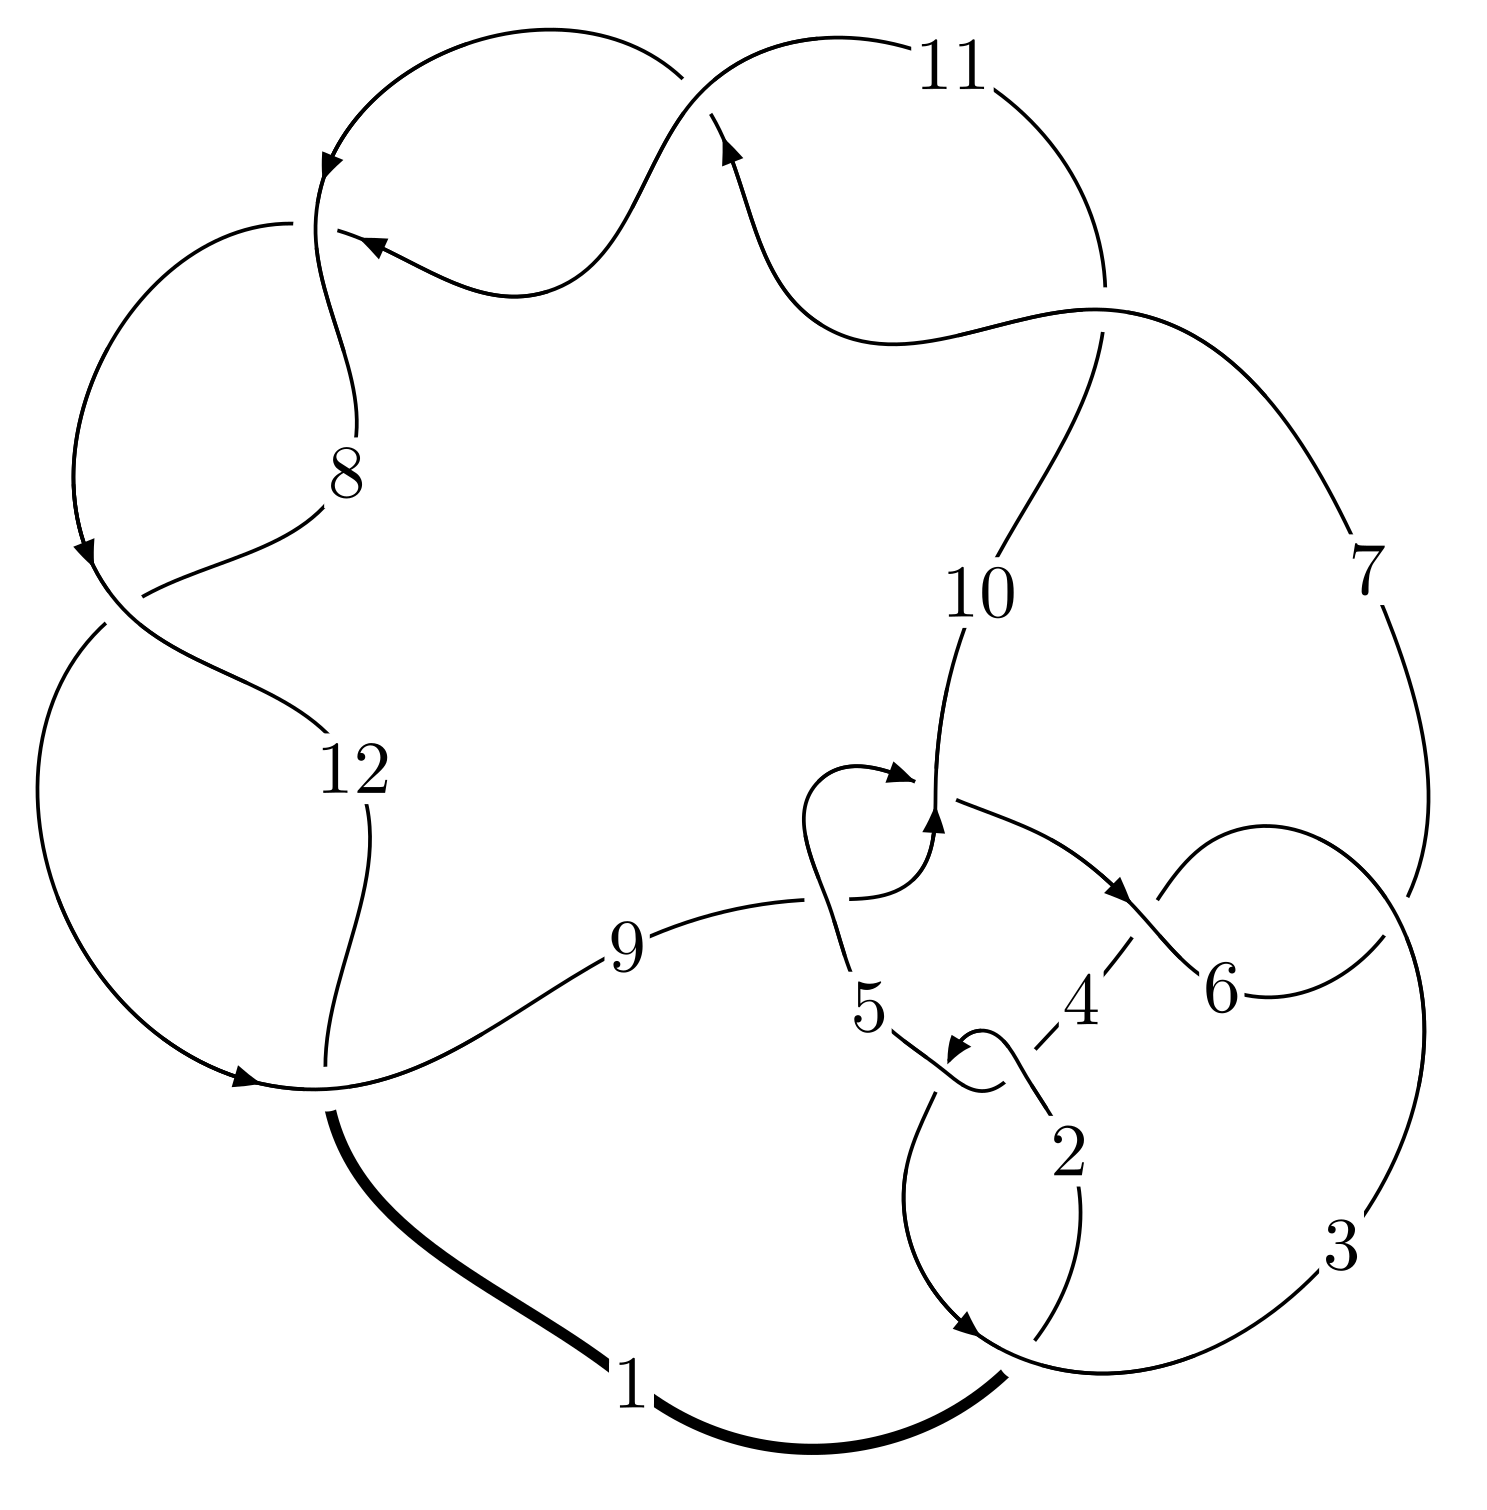
\includegraphics[width=112pt]{../../../GIT/diagram.site/Diagrams/png/2202_12n_0113.png}\\
\ \ \ A knot diagram\footnotemark}&
\allowdisplaybreaks
\textbf{Linearized knot diagam} \\
\cline{2-2}
 &
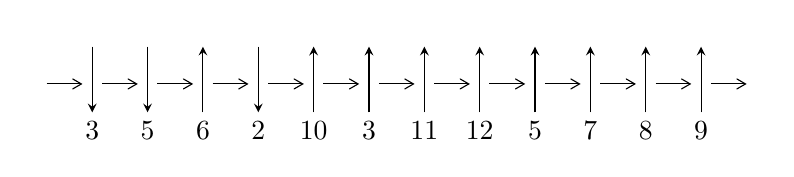
\begin{tikzpicture}[x=20pt, y=17pt]
	% nodes
	\node (C0) at (0, 0) {};
	\node (C1) at (1, 0) {};
	\node (C1U) at (1, +1) {};
	\node (C1D) at (1, -1) {3};

	\node (C2) at (2, 0) {};
	\node (C2U) at (2, +1) {};
	\node (C2D) at (2, -1) {5};

	\node (C3) at (3, 0) {};
	\node (C3U) at (3, +1) {};
	\node (C3D) at (3, -1) {6};

	\node (C4) at (4, 0) {};
	\node (C4U) at (4, +1) {};
	\node (C4D) at (4, -1) {2};

	\node (C5) at (5, 0) {};
	\node (C5U) at (5, +1) {};
	\node (C5D) at (5, -1) {10};

	\node (C6) at (6, 0) {};
	\node (C6U) at (6, +1) {};
	\node (C6D) at (6, -1) {3};

	\node (C7) at (7, 0) {};
	\node (C7U) at (7, +1) {};
	\node (C7D) at (7, -1) {11};

	\node (C8) at (8, 0) {};
	\node (C8U) at (8, +1) {};
	\node (C8D) at (8, -1) {12};

	\node (C9) at (9, 0) {};
	\node (C9U) at (9, +1) {};
	\node (C9D) at (9, -1) {5};

	\node (C10) at (10, 0) {};
	\node (C10U) at (10, +1) {};
	\node (C10D) at (10, -1) {7};

	\node (C11) at (11, 0) {};
	\node (C11U) at (11, +1) {};
	\node (C11D) at (11, -1) {8};

	\node (C12) at (12, 0) {};
	\node (C12U) at (12, +1) {};
	\node (C12D) at (12, -1) {9};
	\node (C13) at (13, 0) {};

	% arrows
	\draw[->,>={angle 60}]
	(C0) edge (C1) (C1) edge (C2) (C2) edge (C3) (C3) edge (C4) (C4) edge (C5) (C5) edge (C6) (C6) edge (C7) (C7) edge (C8) (C8) edge (C9) (C9) edge (C10) (C10) edge (C11) (C11) edge (C12) (C12) edge (C13) ;	\draw[->,>=stealth]
	(C1U) edge (C1D) (C2U) edge (C2D) (C3D) edge (C3U) (C4U) edge (C4D) (C5D) edge (C5U) (C6D) edge (C6U) (C7D) edge (C7U) (C8D) edge (C8U) (C9D) edge (C9U) (C10D) edge (C10U) (C11D) edge (C11U) (C12D) edge (C12U) ;
	\end{tikzpicture} \\
\hhline{~~} \\& 
\textbf{Solving Sequence} \\ \cline{2-2} 
 &
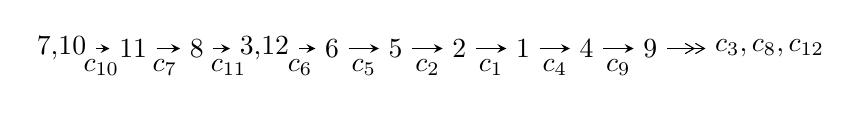
\begin{tikzpicture}[x=23pt, y=7pt]
	% node
	\node (A0) at (-1/8, 0) {7,10};
	\node (A1) at (1, 0) {11};
	\node (A2) at (2, 0) {8};
	\node (A3) at (49/16, 0) {3,12};
	\node (A4) at (33/8, 0) {6};
	\node (A5) at (41/8, 0) {5};
	\node (A6) at (49/8, 0) {2};
	\node (A7) at (57/8, 0) {1};
	\node (A8) at (65/8, 0) {4};
	\node (A9) at (73/8, 0) {9};
	\node (C1) at (1/2, -1) {$c_{10}$};
	\node (C2) at (3/2, -1) {$c_{7}$};
	\node (C3) at (5/2, -1) {$c_{11}$};
	\node (C4) at (29/8, -1) {$c_{6}$};
	\node (C5) at (37/8, -1) {$c_{5}$};
	\node (C6) at (45/8, -1) {$c_{2}$};
	\node (C7) at (53/8, -1) {$c_{1}$};
	\node (C8) at (61/8, -1) {$c_{4}$};
	\node (C9) at (69/8, -1) {$c_{9}$};
	\node (A10) at (11, 0) {$c_{3},c_{8},c_{12}$};

	% edge
	\draw[->,>=stealth]	
	(A0) edge (A1) (A1) edge (A2) (A2) edge (A3) (A3) edge (A4) (A4) edge (A5) (A5) edge (A6) (A6) edge (A7) (A7) edge (A8) (A8) edge (A9) ;
	\draw[->>,>={angle 60}]	
	(A9) edge (A10);
\end{tikzpicture} \\ 

\end{tabular} \\

\footnotetext{
The image of knot diagram is generated by the software ``\textbf{Draw programme}" developed by Andrew Bartholomew(\url{http://www.layer8.co.uk/maths/draw/index.htm\#Running-draw}), where we modified some parts for our purpose(\url{https://github.com/CATsTAILs/LinksPainter}).
}\phantom \\ \newline 
\centering \textbf{Ideals for irreducible components\footnotemark of $X_{\text{par}}$} 
 
\begin{align*}
I^u_{1}&=\langle 
-647354734 u^{28}+978901627 u^{27}+\cdots+206032449 b-1184912620,\\
\phantom{I^u_{1}}&\phantom{= \langle  }-64940111 u^{28}+106362659 u^{27}+\cdots+206032449 a+214765723,\;u^{29}-2 u^{28}+\cdots+u-1\rangle \\
I^u_{2}&=\langle 
u^2+b- u-2,\;a,\;u^3- u^2-2 u+1\rangle \\
\\
\end{align*}
\raggedright * 2 irreducible components of $\dim_{\mathbb{C}}=0$, with total 32 representations.\\
\footnotetext{All coefficients of polynomials are rational numbers. But the coefficients are sometimes approximated in decimal forms when there is not enough margin.}
\newpage
\renewcommand{\arraystretch}{1}
\centering \section*{I. $I^u_{1}= \langle -6.47\times10^{8} u^{28}+9.79\times10^{8} u^{27}+\cdots+2.06\times10^{8} b-1.18\times10^{9},\;-6.49\times10^{7} u^{28}+1.06\times10^{8} u^{27}+\cdots+2.06\times10^{8} a+2.15\times10^{8},\;u^{29}-2 u^{28}+\cdots+u-1 \rangle$}
\flushleft \textbf{(i) Arc colorings}\\
\begin{tabular}{m{7pt} m{180pt} m{7pt} m{180pt} }
\flushright $a_{7}=$&$\begin{pmatrix}0\\u\end{pmatrix}$ \\
\flushright $a_{10}=$&$\begin{pmatrix}1\\0\end{pmatrix}$ \\
\flushright $a_{11}=$&$\begin{pmatrix}1\\- u^2\end{pmatrix}$ \\
\flushright $a_{8}=$&$\begin{pmatrix}u\\- u^3+u\end{pmatrix}$ \\
\flushright $a_{3}=$&$\begin{pmatrix}0.315194 u^{28}-0.516242 u^{27}+\cdots+1.82950 u-1.04239\\3.14200 u^{28}-4.75120 u^{27}+\cdots+6.60148 u+5.75110\end{pmatrix}$ \\
\flushright $a_{12}=$&$\begin{pmatrix}- u^2+1\\u^4-2 u^2\end{pmatrix}$ \\
\flushright $a_{6}=$&$\begin{pmatrix}-0.839121 u^{28}+0.843763 u^{27}+\cdots-1.98749 u-0.119530\\0.215298 u^{28}-0.607510 u^{27}+\cdots+1.52402 u+1.00763\end{pmatrix}$ \\
\flushright $a_{5}=$&$\begin{pmatrix}-1.05442 u^{28}+1.45127 u^{27}+\cdots-3.51151 u-1.12716\\0.215298 u^{28}-0.607510 u^{27}+\cdots+1.52402 u+1.00763\end{pmatrix}$ \\
\flushright $a_{2}=$&$\begin{pmatrix}2.20636 u^{28}-2.61370 u^{27}+\cdots+2.80648 u-0.296715\\3.57260 u^{28}-4.96622 u^{27}+\cdots+5.64951 u+5.76636\end{pmatrix}$ \\
\flushright $a_{1}=$&$\begin{pmatrix}- u^4+3 u^2-1\\u^6-4 u^4+3 u^2\end{pmatrix}$ \\
\flushright $a_{4}=$&$\begin{pmatrix}3.16326 u^{28}-3.35382 u^{27}+\cdots-0.465478 u+0.381491\\3.74875 u^{28}-5.35442 u^{27}+\cdots+5.78774 u+6.35427\end{pmatrix}$ \\
\flushright $a_{9}=$&$\begin{pmatrix}- u^3+2 u\\u^5-3 u^3+u\end{pmatrix}$\\&\end{tabular}
\flushleft \textbf{(ii) Obstruction class $= -1$}\\~\\
\flushleft \textbf{(iii) Cusp Shapes $= -\frac{3792380055}{68677483} u^{28}+\frac{5628748625}{68677483} u^{27}+\cdots-\frac{5070709179}{68677483} u-\frac{6687860995}{68677483}$}\\~\\
\newpage\renewcommand{\arraystretch}{1}
\flushleft \textbf{(iv) u-Polynomials at the component}\newline \\
\begin{tabular}{m{50pt}|m{274pt}}
Crossings & \hspace{64pt}u-Polynomials at each crossing \\
\hline $$\begin{aligned}c_{1}\end{aligned}$$&$\begin{aligned}
&u^{29}+30 u^{28}+\cdots+530 u+1
\end{aligned}$\\
\hline $$\begin{aligned}c_{2},c_{4}\end{aligned}$$&$\begin{aligned}
&u^{29}-4 u^{28}+\cdots+18 u-1
\end{aligned}$\\
\hline $$\begin{aligned}c_{3},c_{6}\end{aligned}$$&$\begin{aligned}
&u^{29}+5 u^{28}+\cdots+84 u-8
\end{aligned}$\\
\hline $$\begin{aligned}c_{5},c_{9}\end{aligned}$$&$\begin{aligned}
&u^{29}+2 u^{28}+\cdots- u-1
\end{aligned}$\\
\hline $$\begin{aligned}c_{7},c_{8},c_{10}\\c_{11},c_{12}\end{aligned}$$&$\begin{aligned}
&u^{29}-2 u^{28}+\cdots+u-1
\end{aligned}$\\
\hline
\end{tabular}\\~\\
\newpage\renewcommand{\arraystretch}{1}
\flushleft \textbf{(v) Riley Polynomials at the component}\newline \\
\begin{tabular}{m{50pt}|m{274pt}}
Crossings & \hspace{64pt}Riley Polynomials at each crossing \\
\hline $$\begin{aligned}c_{1}\end{aligned}$$&$\begin{aligned}
&y^{29}-58 y^{28}+\cdots+261102 y-1
\end{aligned}$\\
\hline $$\begin{aligned}c_{2},c_{4}\end{aligned}$$&$\begin{aligned}
&y^{29}-30 y^{28}+\cdots+530 y-1
\end{aligned}$\\
\hline $$\begin{aligned}c_{3},c_{6}\end{aligned}$$&$\begin{aligned}
&y^{29}+21 y^{28}+\cdots+2256 y-64
\end{aligned}$\\
\hline $$\begin{aligned}c_{5},c_{9}\end{aligned}$$&$\begin{aligned}
&y^{29}+30 y^{27}+\cdots+9 y-1
\end{aligned}$\\
\hline $$\begin{aligned}c_{7},c_{8},c_{10}\\c_{11},c_{12}\end{aligned}$$&$\begin{aligned}
&y^{29}-36 y^{28}+\cdots+9 y-1
\end{aligned}$\\
\hline
\end{tabular}\\~\\
\newpage\flushleft \textbf{(vi) Complex Volumes and Cusp Shapes}
$$\begin{array}{c|c|c}  
\text{Solutions to }I^u_{1}& \I (\text{vol} + \sqrt{-1}CS) & \text{Cusp shape}\\
 \hline 
\begin{aligned}
u &= -0.871800 + 0.572952 I \\
a &= -1.34659 + 0.79448 I \\
b &= -1.48468 - 0.59106 I\end{aligned}
 & -6.35449 - 8.78908 I & \phantom{-}6.18505 + 6.40374 I \\ \hline\begin{aligned}
u &= -0.871800 - 0.572952 I \\
a &= -1.34659 - 0.79448 I \\
b &= -1.48468 + 0.59106 I\end{aligned}
 & -6.35449 + 8.78908 I & \phantom{-}6.18505 - 6.40374 I \\ \hline\begin{aligned}
u &= \phantom{-}0.915102 + 0.577424 I \\
a &= -0.630350 - 1.126710 I \\
b &= -1.262120 - 0.106799 I\end{aligned}
 & -6.10118 + 0.29510 I & \phantom{-}5.18889 - 1.16439 I \\ \hline\begin{aligned}
u &= \phantom{-}0.915102 - 0.577424 I \\
a &= -0.630350 + 1.126710 I \\
b &= -1.262120 + 0.106799 I\end{aligned}
 & -6.10118 - 0.29510 I & \phantom{-}5.18889 + 1.16439 I \\ \hline\begin{aligned}
u &= -1.14574\phantom{ +0.000000I} \\
a &= \phantom{-}0.540876\phantom{ +0.000000I} \\
b &= -0.0550040\phantom{ +0.000000I}\end{aligned}
 & \phantom{-}5.50698\phantom{ +0.000000I} & \phantom{-}18.3420\phantom{ +0.000000I} \\ \hline\begin{aligned}
u &= -0.020234 + 0.793792 I \\
a &= \phantom{-}1.86337 - 0.55939 I \\
b &= \phantom{-}1.41720 - 0.34042 I\end{aligned}
 & -8.92001 + 4.25864 I & \phantom{-}2.72812 - 2.59912 I \\ \hline\begin{aligned}
u &= -0.020234 - 0.793792 I \\
a &= \phantom{-}1.86337 + 0.55939 I \\
b &= \phantom{-}1.41720 + 0.34042 I\end{aligned}
 & -8.92001 - 4.25864 I & \phantom{-}2.72812 + 2.59912 I \\ \hline\begin{aligned}
u &= -0.699728 + 0.338099 I \\
a &= \phantom{-}1.36237 - 1.32693 I \\
b &= \phantom{-}0.968494 + 0.555673 I\end{aligned}
 & \phantom{-}0.16525 - 3.96735 I & \phantom{-}8.32283 + 8.62955 I \\ \hline\begin{aligned}
u &= -0.699728 - 0.338099 I \\
a &= \phantom{-}1.36237 + 1.32693 I \\
b &= \phantom{-}0.968494 - 0.555673 I\end{aligned}
 & \phantom{-}0.16525 + 3.96735 I & \phantom{-}8.32283 - 8.62955 I \\ \hline\begin{aligned}
u &= \phantom{-}0.680274 + 0.194448 I \\
a &= \phantom{-}0.272779 + 0.785923 I \\
b &= \phantom{-}1.128350 - 0.317013 I\end{aligned}
 & \phantom{-}0.478397 + 0.446224 I & \phantom{-}9.33081 - 0.68417 I\\
 \hline 
 \end{array}$$\newpage$$\begin{array}{c|c|c}  
\text{Solutions to }I^u_{1}& \I (\text{vol} + \sqrt{-1}CS) & \text{Cusp shape}\\
 \hline 
\begin{aligned}
u &= \phantom{-}0.680274 - 0.194448 I \\
a &= \phantom{-}0.272779 - 0.785923 I \\
b &= \phantom{-}1.128350 + 0.317013 I\end{aligned}
 & \phantom{-}0.478397 - 0.446224 I & \phantom{-}9.33081 + 0.68417 I \\ \hline\begin{aligned}
u &= -0.439691 + 0.314107 I \\
a &= -1.42146 - 2.04429 I \\
b &= -0.346882 - 0.207064 I\end{aligned}
 & -2.81354 - 1.22096 I & \phantom{-}1.65575 + 5.11958 I \\ \hline\begin{aligned}
u &= -0.439691 - 0.314107 I \\
a &= -1.42146 + 2.04429 I \\
b &= -0.346882 + 0.207064 I\end{aligned}
 & -2.81354 + 1.22096 I & \phantom{-}1.65575 - 5.11958 I \\ \hline\begin{aligned}
u &= \phantom{-}0.536642\phantom{ +0.000000I} \\
a &= -0.443928\phantom{ +0.000000I} \\
b &= -3.69157\phantom{ +0.000000I}\end{aligned}
 & -0.846423\phantom{ +0.000000I} & \phantom{-}87.1400\phantom{ +0.000000I} \\ \hline\begin{aligned}
u &= \phantom{-}1.55407 + 0.03946 I \\
a &= \phantom{-}0.992776 - 0.855482 I \\
b &= \phantom{-}0.766756 + 0.115816 I\end{aligned}
 & \phantom{-}3.99647 + 2.19066 I & \phantom{-0.000000 } 0 \\ \hline\begin{aligned}
u &= \phantom{-}1.55407 - 0.03946 I \\
a &= \phantom{-}0.992776 + 0.855482 I \\
b &= \phantom{-}0.766756 - 0.115816 I\end{aligned}
 & \phantom{-}3.99647 - 2.19066 I & \phantom{-0.000000 } 0 \\ \hline\begin{aligned}
u &= -1.59090\phantom{ +0.000000I} \\
a &= \phantom{-}0.405019\phantom{ +0.000000I} \\
b &= \phantom{-}3.31575\phantom{ +0.000000I}\end{aligned}
 & \phantom{-}6.62367\phantom{ +0.000000I} & \phantom{-}25.1550\phantom{ +0.000000I} \\ \hline\begin{aligned}
u &= \phantom{-}0.394545\phantom{ +0.000000I} \\
a &= -0.532583\phantom{ +0.000000I} \\
b &= \phantom{-}0.353791\phantom{ +0.000000I}\end{aligned}
 & \phantom{-}0.662854\phantom{ +0.000000I} & \phantom{-}15.1320\phantom{ +0.000000I} \\ \hline\begin{aligned}
u &= -0.079696 + 0.381721 I \\
a &= -2.52365 + 0.46294 I \\
b &= -0.986678 + 0.376786 I\end{aligned}
 & -1.55597 + 1.38501 I & \phantom{-}1.25824 - 2.95729 I \\ \hline\begin{aligned}
u &= -0.079696 - 0.381721 I \\
a &= -2.52365 - 0.46294 I \\
b &= -0.986678 - 0.376786 I\end{aligned}
 & -1.55597 - 1.38501 I & \phantom{-}1.25824 + 2.95729 I\\
 \hline 
 \end{array}$$\newpage$$\begin{array}{c|c|c}  
\text{Solutions to }I^u_{1}& \I (\text{vol} + \sqrt{-1}CS) & \text{Cusp shape}\\
 \hline 
\begin{aligned}
u &= \phantom{-}1.61444 + 0.08862 I \\
a &= -0.653048 - 0.970484 I \\
b &= -1.011500 + 0.774939 I\end{aligned}
 & \phantom{-}8.13246 + 5.52553 I & \phantom{-0.000000 } 0 \\ \hline\begin{aligned}
u &= \phantom{-}1.61444 - 0.08862 I \\
a &= -0.653048 + 0.970484 I \\
b &= -1.011500 - 0.774939 I\end{aligned}
 & \phantom{-}8.13246 - 5.52553 I & \phantom{-0.000000 } 0 \\ \hline\begin{aligned}
u &= -1.62438 + 0.04713 I \\
a &= -0.178840 + 0.450917 I \\
b &= -1.17354 - 1.05585 I\end{aligned}
 & \phantom{-}8.53322 - 1.28090 I & \phantom{-0.000000 } 0 \\ \hline\begin{aligned}
u &= -1.62438 - 0.04713 I \\
a &= -0.178840 - 0.450917 I \\
b &= -1.17354 + 1.05585 I\end{aligned}
 & \phantom{-}8.53322 + 1.28090 I & \phantom{-0.000000 } 0 \\ \hline\begin{aligned}
u &= \phantom{-}1.66621 + 0.17240 I \\
a &= \phantom{-}0.679212 + 0.775786 I \\
b &= \phantom{-}1.53044 - 0.82697 I\end{aligned}
 & \phantom{-}2.31087 + 11.70390 I & \phantom{-0.000000 } 0 \\ \hline\begin{aligned}
u &= \phantom{-}1.66621 - 0.17240 I \\
a &= \phantom{-}0.679212 - 0.775786 I \\
b &= \phantom{-}1.53044 + 0.82697 I\end{aligned}
 & \phantom{-}2.31087 - 11.70390 I & \phantom{-0.000000 } 0 \\ \hline\begin{aligned}
u &= -1.68491 + 0.18549 I \\
a &= \phantom{-}0.244062 - 0.717045 I \\
b &= \phantom{-}1.081240 + 0.132670 I\end{aligned}
 & \phantom{-}2.80677 - 3.35130 I & \phantom{-0.000000 } 0 \\ \hline\begin{aligned}
u &= -1.68491 - 0.18549 I \\
a &= \phantom{-}0.244062 + 0.717045 I \\
b &= \phantom{-}1.081240 - 0.132670 I\end{aligned}
 & \phantom{-}2.80677 + 3.35130 I & \phantom{-0.000000 } 0 \\ \hline\begin{aligned}
u &= \phantom{-}1.78613\phantom{ +0.000000I} \\
a &= -0.290652\phantom{ +0.000000I} \\
b &= -0.177069\phantom{ +0.000000I}\end{aligned}
 & \phantom{-}16.3052\phantom{ +0.000000I} & \phantom{-0.000000 } 0\\
 \hline 
 \end{array}$$\newpage\newpage\renewcommand{\arraystretch}{1}
\centering \section*{II. $I^u_{2}= \langle u^2+b- u-2,\;a,\;u^3- u^2-2 u+1 \rangle$}
\flushleft \textbf{(i) Arc colorings}\\
\begin{tabular}{m{7pt} m{180pt} m{7pt} m{180pt} }
\flushright $a_{7}=$&$\begin{pmatrix}0\\u\end{pmatrix}$ \\
\flushright $a_{10}=$&$\begin{pmatrix}1\\0\end{pmatrix}$ \\
\flushright $a_{11}=$&$\begin{pmatrix}1\\- u^2\end{pmatrix}$ \\
\flushright $a_{8}=$&$\begin{pmatrix}u\\- u^2- u+1\end{pmatrix}$ \\
\flushright $a_{3}=$&$\begin{pmatrix}0\\- u^2+u+2\end{pmatrix}$ \\
\flushright $a_{12}=$&$\begin{pmatrix}- u^2+1\\u^2+u-1\end{pmatrix}$ \\
\flushright $a_{6}=$&$\begin{pmatrix}0\\u\end{pmatrix}$ \\
\flushright $a_{5}=$&$\begin{pmatrix}- u\\u\end{pmatrix}$ \\
\flushright $a_{2}=$&$\begin{pmatrix}u\\- u^2+2\end{pmatrix}$ \\
\flushright $a_{1}=$&$\begin{pmatrix}u\\- u\end{pmatrix}$ \\
\flushright $a_{4}=$&$\begin{pmatrix}0\\- u^2+u+2\end{pmatrix}$ \\
\flushright $a_{9}=$&$\begin{pmatrix}- u^2+1\\u^2\end{pmatrix}$\\&\end{tabular}
\flushleft \textbf{(ii) Obstruction class $= 1$}\\~\\
\flushleft \textbf{(iii) Cusp Shapes $= 8 u^2-7 u-14$}\\~\\
\newpage\renewcommand{\arraystretch}{1}
\flushleft \textbf{(iv) u-Polynomials at the component}\newline \\
\begin{tabular}{m{50pt}|m{274pt}}
Crossings & \hspace{64pt}u-Polynomials at each crossing \\
\hline $$\begin{aligned}c_{1},c_{2}\end{aligned}$$&$\begin{aligned}
&(u-1)^3
\end{aligned}$\\
\hline $$\begin{aligned}c_{3},c_{6}\end{aligned}$$&$\begin{aligned}
&u^3
\end{aligned}$\\
\hline $$\begin{aligned}c_{4}\end{aligned}$$&$\begin{aligned}
&(u+1)^3
\end{aligned}$\\
\hline $$\begin{aligned}c_{5},c_{7},c_{8}\end{aligned}$$&$\begin{aligned}
&u^3+u^2-2 u-1
\end{aligned}$\\
\hline $$\begin{aligned}c_{9},c_{10},c_{11}\\c_{12}\end{aligned}$$&$\begin{aligned}
&u^3- u^2-2 u+1
\end{aligned}$\\
\hline
\end{tabular}\\~\\
\newpage\renewcommand{\arraystretch}{1}
\flushleft \textbf{(v) Riley Polynomials at the component}\newline \\
\begin{tabular}{m{50pt}|m{274pt}}
Crossings & \hspace{64pt}Riley Polynomials at each crossing \\
\hline $$\begin{aligned}c_{1},c_{2},c_{4}\end{aligned}$$&$\begin{aligned}
&(y-1)^3
\end{aligned}$\\
\hline $$\begin{aligned}c_{3},c_{6}\end{aligned}$$&$\begin{aligned}
&y^3
\end{aligned}$\\
\hline $$\begin{aligned}c_{5},c_{7},c_{8}\\c_{9},c_{10},c_{11}\\c_{12}\end{aligned}$$&$\begin{aligned}
&y^3-5 y^2+6 y-1
\end{aligned}$\\
\hline
\end{tabular}\\~\\
\newpage\flushleft \textbf{(vi) Complex Volumes and Cusp Shapes}
$$\begin{array}{c|c|c}  
\text{Solutions to }I^u_{2}& \I (\text{vol} + \sqrt{-1}CS) & \text{Cusp shape}\\
 \hline 
\begin{aligned}
u &= -1.24698\phantom{ +0.000000I} \\
a &= \phantom{-0.000000 } 0 \\
b &= -0.801938\phantom{ +0.000000I}\end{aligned}
 & \phantom{-}4.69981\phantom{ +0.000000I} & \phantom{-}7.16850\phantom{ +0.000000I} \\ \hline\begin{aligned}
u &= \phantom{-}0.445042\phantom{ +0.000000I} \\
a &= \phantom{-0.000000 } 0 \\
b &= \phantom{-}2.24698\phantom{ +0.000000I}\end{aligned}
 & -0.939962\phantom{ +0.000000I} & -15.5310\phantom{ +0.000000I} \\ \hline\begin{aligned}
u &= \phantom{-}1.80194\phantom{ +0.000000I} \\
a &= \phantom{-0.000000 } 0 \\
b &= \phantom{-}0.554958\phantom{ +0.000000I}\end{aligned}
 & \phantom{-}15.9794\phantom{ +0.000000I} & -0.637730\phantom{ +0.000000I}\\
 \hline 
 \end{array}$$\newpage
\newpage\renewcommand{\arraystretch}{1}
\centering \section*{ III. u-Polynomials}
\begin{tabular}{m{50pt}|m{274pt}}
Crossings & \hspace{64pt}u-Polynomials at each crossing \\
\hline $$\begin{aligned}c_{1}\end{aligned}$$&$\begin{aligned}
&((u-1)^3)(u^{29}+30 u^{28}+\cdots+530 u+1)
\end{aligned}$\\
\hline $$\begin{aligned}c_{2}\end{aligned}$$&$\begin{aligned}
&((u-1)^3)(u^{29}-4 u^{28}+\cdots+18 u-1)
\end{aligned}$\\
\hline $$\begin{aligned}c_{3},c_{6}\end{aligned}$$&$\begin{aligned}
&u^3(u^{29}+5 u^{28}+\cdots+84 u-8)
\end{aligned}$\\
\hline $$\begin{aligned}c_{4}\end{aligned}$$&$\begin{aligned}
&((u+1)^3)(u^{29}-4 u^{28}+\cdots+18 u-1)
\end{aligned}$\\
\hline $$\begin{aligned}c_{5}\end{aligned}$$&$\begin{aligned}
&(u^3+u^2-2 u-1)(u^{29}+2 u^{28}+\cdots- u-1)
\end{aligned}$\\
\hline $$\begin{aligned}c_{7},c_{8}\end{aligned}$$&$\begin{aligned}
&(u^3+u^2-2 u-1)(u^{29}-2 u^{28}+\cdots+u-1)
\end{aligned}$\\
\hline $$\begin{aligned}c_{9}\end{aligned}$$&$\begin{aligned}
&(u^3- u^2-2 u+1)(u^{29}+2 u^{28}+\cdots- u-1)
\end{aligned}$\\
\hline $$\begin{aligned}c_{10},c_{11},c_{12}\end{aligned}$$&$\begin{aligned}
&(u^3- u^2-2 u+1)(u^{29}-2 u^{28}+\cdots+u-1)
\end{aligned}$\\
\hline
\end{tabular}\newpage\renewcommand{\arraystretch}{1}
\centering \section*{ IV. Riley Polynomials}
\begin{tabular}{m{50pt}|m{274pt}}
Crossings & \hspace{64pt}Riley Polynomials at each crossing \\
\hline $$\begin{aligned}c_{1}\end{aligned}$$&$\begin{aligned}
&((y-1)^3)(y^{29}-58 y^{28}+\cdots+261102 y-1)
\end{aligned}$\\
\hline $$\begin{aligned}c_{2},c_{4}\end{aligned}$$&$\begin{aligned}
&((y-1)^3)(y^{29}-30 y^{28}+\cdots+530 y-1)
\end{aligned}$\\
\hline $$\begin{aligned}c_{3},c_{6}\end{aligned}$$&$\begin{aligned}
&y^3(y^{29}+21 y^{28}+\cdots+2256 y-64)
\end{aligned}$\\
\hline $$\begin{aligned}c_{5},c_{9}\end{aligned}$$&$\begin{aligned}
&(y^3-5 y^2+6 y-1)(y^{29}+30 y^{27}+\cdots+9 y-1)
\end{aligned}$\\
\hline $$\begin{aligned}c_{7},c_{8},c_{10}\\c_{11},c_{12}\end{aligned}$$&$\begin{aligned}
&(y^3-5 y^2+6 y-1)(y^{29}-36 y^{28}+\cdots+9 y-1)
\end{aligned}$\\
\hline
\end{tabular}
\vskip 2pc
\end{document}